\chapter{Uživatelské testování}

\section{System Usability Scale (SUS)}
System Usability Scale je jednoduchý test na přívětivost uživatelského rozhraní aplikace. Cílem tohoto testování je seznámit uživatele s aplikací a pak mu položit 10 otázek, které SUS definuje. Na základě odpovědí na tyto otázky je pak spočteno skóre uživatelské přívětivosti. Aby testování bylo objektivní, je potřeba aplikaci testovat na osobách, jež se nepodílely na žádné části softwarového vývoje.

Testovaným osobám bude vysvětlen základní princip fungování aplikace a poté jim budou určeny jednoduché úkoly, které musí splnit. Znění těchto úkolů bude úmyslně napsáno velmi obecně a nebudou použity termíny, jež jsou použity v aplikaci. Testovaná osoba pak musí sama přijít na to, jak danou akci provést a díky tomu bude schopna objektivně zhodnotit přívětivost uživatelského rozhraní.

\begin{enumerate}
    \item Zjistěte, které taxony řadíme pod Vyšší rostliny (latinsky Embryophyta).
    \item Pokuste se vyrobit graf podobný grafu na obrázku. Toto uspořádání vrcholů do stromu se nazývá \textbf{dagre}. Konkrétní pořadí vrcholů není důležité.
    \begin{figure}[h]
        \centering
        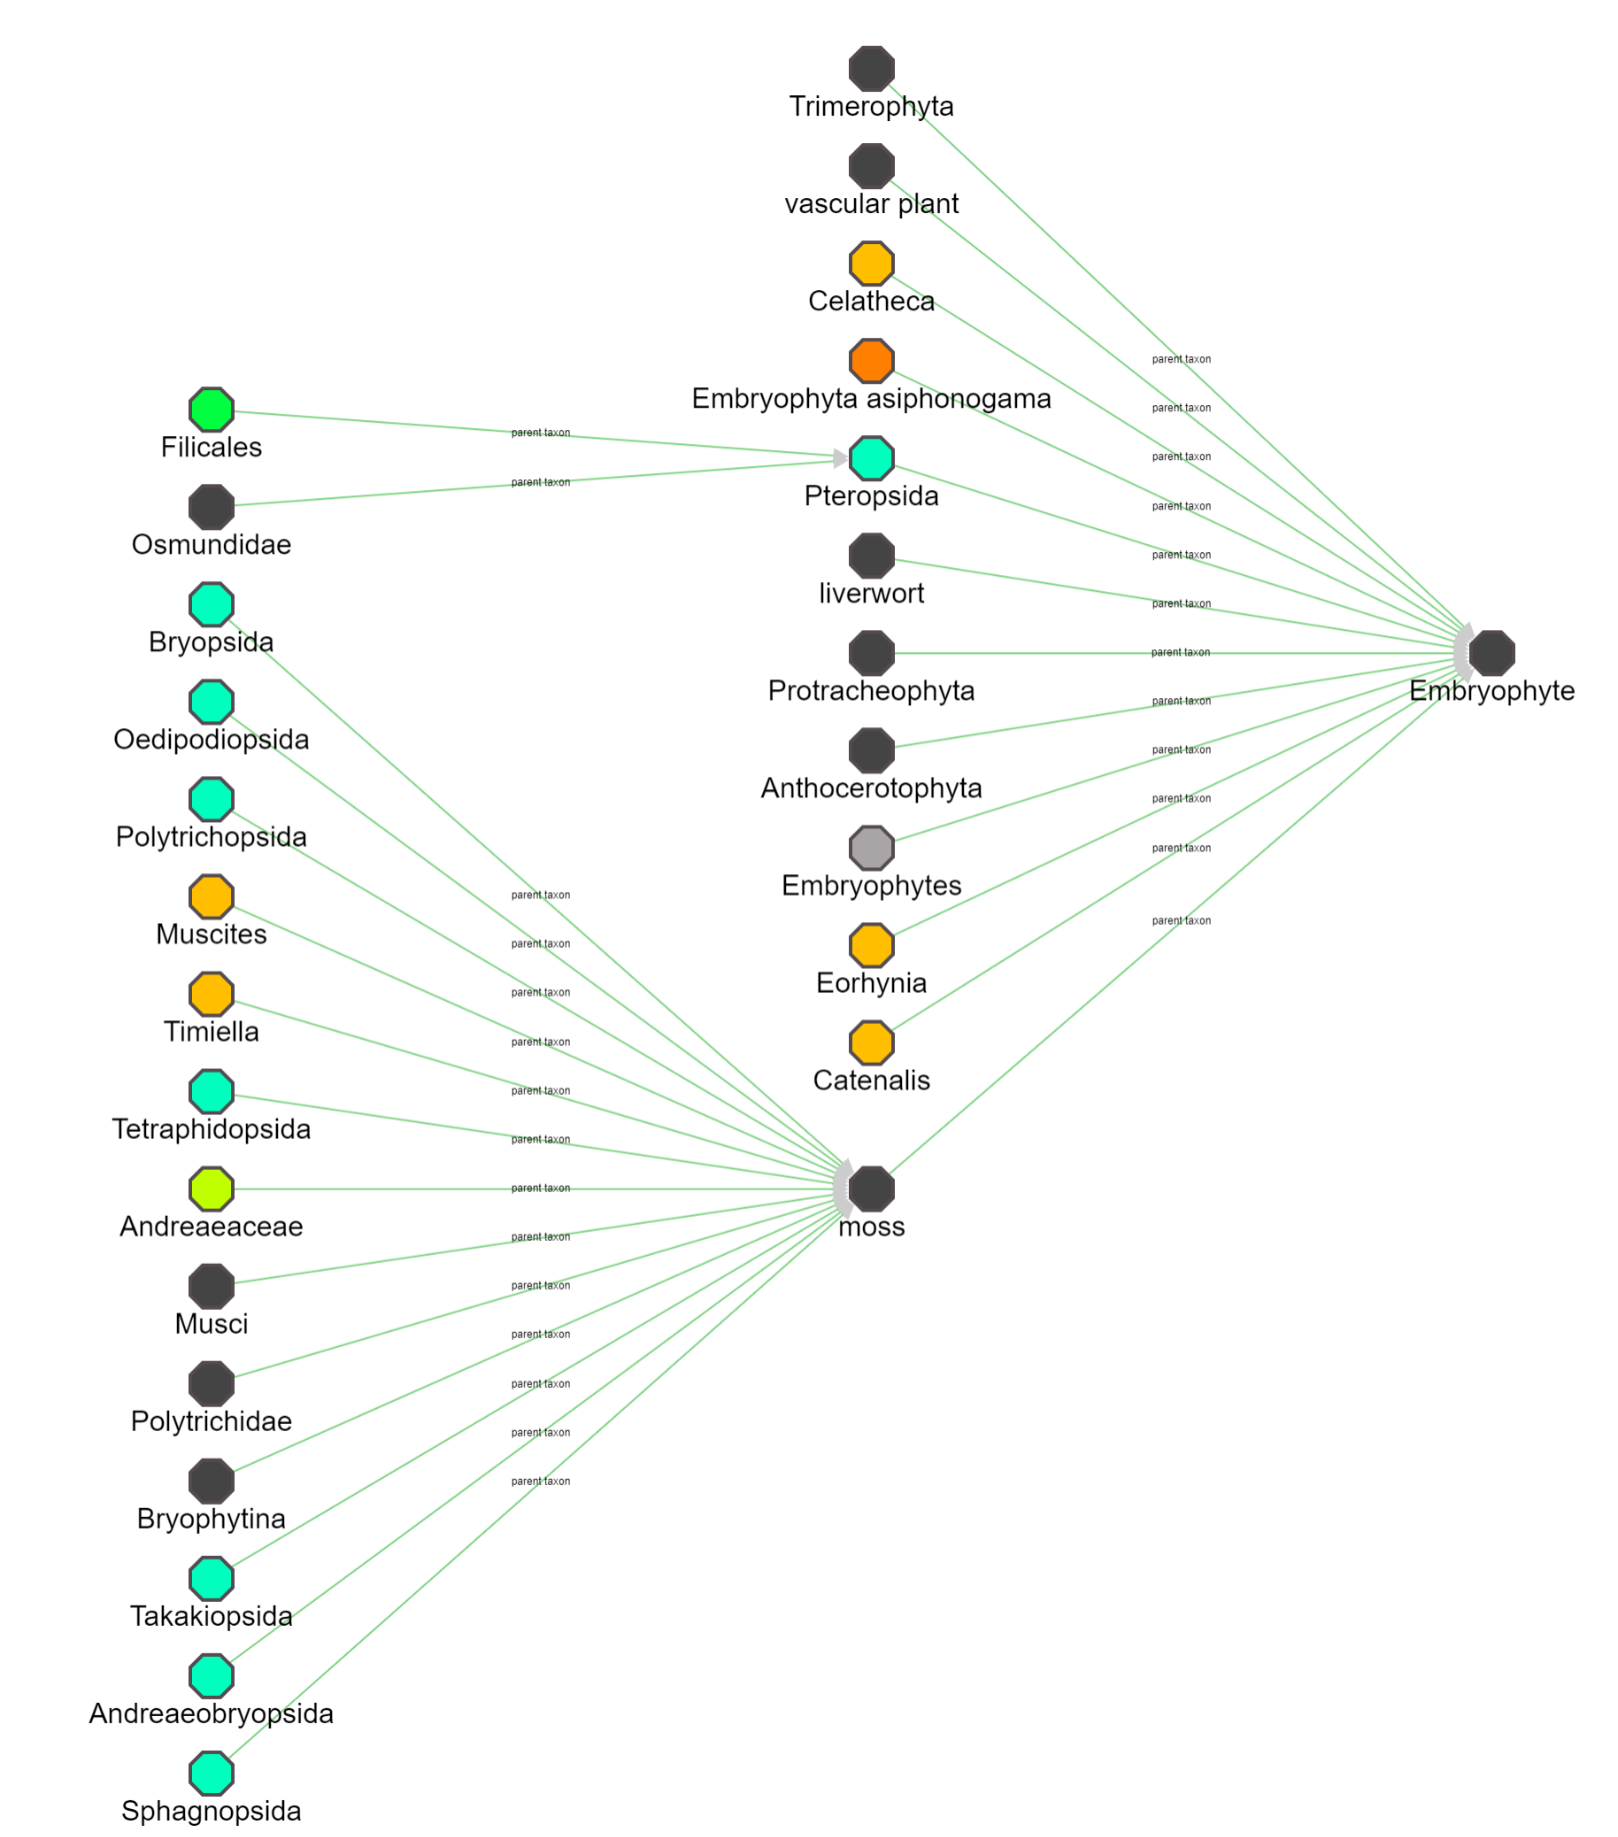
\includegraphics[width=0.5\textwidth]{media/sus-dagre.png}
    \end{figure}
    \item Stáhněte si aktuální graf do souboru, stránku aktualizujte a graf ze souboru opět načtěte.
    \item Nechte si zobrazit ze všech vrcholů jen ty, co mají třídu \uv{genus}.
    \item Bez aktualizace stránky změntě konfiguraci na \uv{Poslanecká sněmovna parlamentu České republiky} a vyberte libovolný uzel.
\end{enumerate}